\documentclass[11pt,a4paper]{article}
\usepackage[margin=2cm]{geometry}
\usepackage{amsmath,amssymb,booktabs,array,graphicx,caption,needspace}
\usepackage[T1]{fontenc}
\usepackage[hidelinks]{hyperref}
\captionsetup{font=small,labelfont=bf,width=0.95\linewidth}
\graphicspath{{../../results/figures/}}
\setlength{\tabcolsep}{3.5pt}
\title{Controlled turbulence-sensitivity study:\\ error of the analytic averages versus $\sigma_X^2$ at fixed distance}
\author{Computed from the repository \texttt{Anand-Ambastha/tf-qkd-private}}
\date{22 October 2026}
\begin{document}\maketitle

\section{Design of the study}
\paragraph{What is varied.} For each fixed total distance $L\in\{80,120,160\}$~km the variance of the log-transmittance $X=\ln(\eta/\eta_0)$, $\eta=\sqrt{\eta_A\eta_B}$, is imposed on a grid $\sigma_X^2\in\{0.005,0.01,0.02,0.05,0.1,0.2,0.3,0.4,0.5,0.6,0.7,0.8\}$, independently of $L$. \textbf{This is a controlled sensitivity study.} The imposed $\sigma_X^2$ values are not claimed to correspond to atmospheric conditions realisable at that distance; the distance enters only through the deterministic transmittance $\eta_0=\sqrt{\eta_{\rm FSO}(L)}$ ($0.0393,\ 0.00757,\ 0.00175$ at $80,120,160$~km, i.e.\ the operating point on the key-rate curve). Where the channel model does tie $\sigma_X^2$ to the atmosphere this is stated below.

\paragraph{Three channel models.}
\begin{itemize}
\item \textbf{LN}: $X\sim\mathcal N(-\sigma_X^2,\sigma_X^2)$ (manuscript model; $\sigma_X^2=\sigma_R^2(L/2)/2$ per arm pair).
\item \textbf{GG}: independent Gamma--Gamma arms, $X=\tfrac12(\ln I_A+\ln I_B)$, $\mathrm{Var}(X)=c_2=\tfrac12[\psi'(\alpha)+\psi'(\beta)]$ with $(\alpha,\beta)$ from the plane-wave Andrews--Phillips formulas (exponent $6/5$ on the Rytov variance, as in the repository code). For each target $\sigma_X^2$ the per-arm Rytov variance is solved from $c_2(\sigma_R^2)=\sigma_X^2$ on the rising branch. \emph{$c_2$ is bounded:} its maximum over all $\sigma_R^2$ is $0.858$ (at $\sigma_R^2\approx52$), because Gamma--Gamma saturates; this fixes the upper end of the grid. The grid values $\ge$ about $0.85$ would correspond to saturated moderate/strong turbulence.
\item \textbf{GG+BB}: as GG, with turbulence-induced long-term beam broadening (which contains beam wander) per arm, $\eta_0\to\eta_0f_{\rm bb}$, $W_{\rm LT}^2=W^2(1+1.63\,\sigma_R^{12/5}\Lambda)$, using the $\sigma_R^2$ solved for GG. Broadening therefore changes the operating point, not the fading statistics. In this study $\sigma_R^2$ and $L$ are independent, so $f_{\rm bb}^2$ is that of an arm of length $L/2$ with the imposed $\sigma_R^2$ (listed in the tables); in a real atmosphere both follow from $C_n^2$.
\end{itemize}
\paragraph{Approximations compared} (all with the repository's analytic derivatives, Appendices A--H of the manuscript): \emph{conventional/mean} $\mathbb E[Q]\simeq Q(\bar\eta)+\tfrac12Q''(\bar\eta)\mathrm{Var}(\eta)$ with $\bar\eta=\mathbb E[\eta]$, $\mathrm{Var}(\eta)=\eta_0^2(1-m_1^2)$, $m_1=\mathbb E[e^X]$; \emph{2nd-order median} $Q(\eta_m)+\tfrac{c_2}{2}\Theta^2Q$; \emph{4th-order median} $Q(\eta_m)+\tfrac{c_2}{2}\Theta^2Q+\tfrac{c_3}{6}\Theta^3Q+\tfrac{c_4+3c_2^2}{24}\Theta^4Q$, all at $\eta_m=\eta_0e^{c_1}$ (cumulants $c_n=2^{1-n}\kappa_n$ for GG, $(-\sigma_X^2,\sigma_X^2,0,0)$ for LN).

\paragraph{References (independent of the formulas).} LN: Simpson quadrature in $X$ over $\mu\pm12\sigma$ (40001 points). GG: numerical convolution of the two arms' Bessel-$K$ log-densities (6001 points each; density norm $=1\pm5\times10^{-10}$ in every case). The transmittance is capped at $1$ in the references; the probability of $\eta>1$ is at most $3.2\times10^{-6}$ in all cases, so the cap does not affect the comparison. Errors are $100(\text{approx}-\text{ref})/\text{ref}$.

\paragraph{Where this study touches realistic conditions.} For the weak class $C_n^2=10^{-17}$ the actual values at $L=80,120,160$~km are $\sigma_X^2=0.086,\,0.181,\,0.307$ (LN, manuscript Table) and $c_2=0.084,\,0.166,\,0.258$ (GG). For the moderate class the Gamma--Gamma channel is saturated, $c_2=0.84$--$0.86$ at all three distances (top of the grid), whereas the log-normal model would give $\sigma_X^2=8.6$--$31$, far outside the tested range. LN results above $\sigma_X^2=0.8$ were not computed.

\section{Turbulence-sensitivity tables}
Tables~\ref{tab:sens-LN}--\ref{tab:sens-GGBB} give all $3\times3\times12$ cases. Table~\ref{tab:thr} condenses the key rate; Table~\ref{tab:thr2} the maximum errors of $e_X$ and $e_Z$.

\begin{table}[htbp]\centering\small
\caption{Secret key rate $R$: $\sigma_X^2$ at which $|{\rm error}|$ first exceeds $0.1\%$ / $1\%$ (log-linear interpolation on the grid; $>0.8$ = not reached within the grid), and the maximum $|{\rm error}|$ [\%] over $0.005\le\sigma_X^2\le0.8$.}
\label{tab:thr}
\begin{tabular}{llccc}\toprule
model & $L$ [km] & mean: $0.1\%$ / $1\%$ / max & 2nd: $0.1\%$ / $1\%$ / max & 4th: $0.1\%$ / $1\%$ / max\\\midrule
%%THR%%\bottomrule\end{tabular}\end{table}

\begin{table}[htbp]\centering\small
\caption{Maximum $|{\rm error}|$ [\%] of $e_X$ and $e_Z$ over $0.005\le\sigma_X^2\le0.8$.}
\label{tab:thr2}
\begin{tabular}{llcccccc}\toprule
 & & \multicolumn{3}{c}{$e_X$} & \multicolumn{3}{c}{$e_Z$}\\\cmidrule(lr){3-5}\cmidrule(lr){6-8}
model & $L$ [km] & mean & 2nd & 4th & mean & 2nd & 4th\\\midrule
%%THR2%%\bottomrule\end{tabular}\end{table}

%%LN%%
%%GG%%
%%GGBB%%

\section{Error versus turbulence strength}
Figures~\ref{fig:LN}--\ref{fig:GGBB}: panels (a) $e_X$, (b) $e_Z$, (c) $R$; colour/marker = approximation, line style = distance; absolute error on a logarithmic axis (signed values are in the tables).
\begin{figure}[htbp]\centering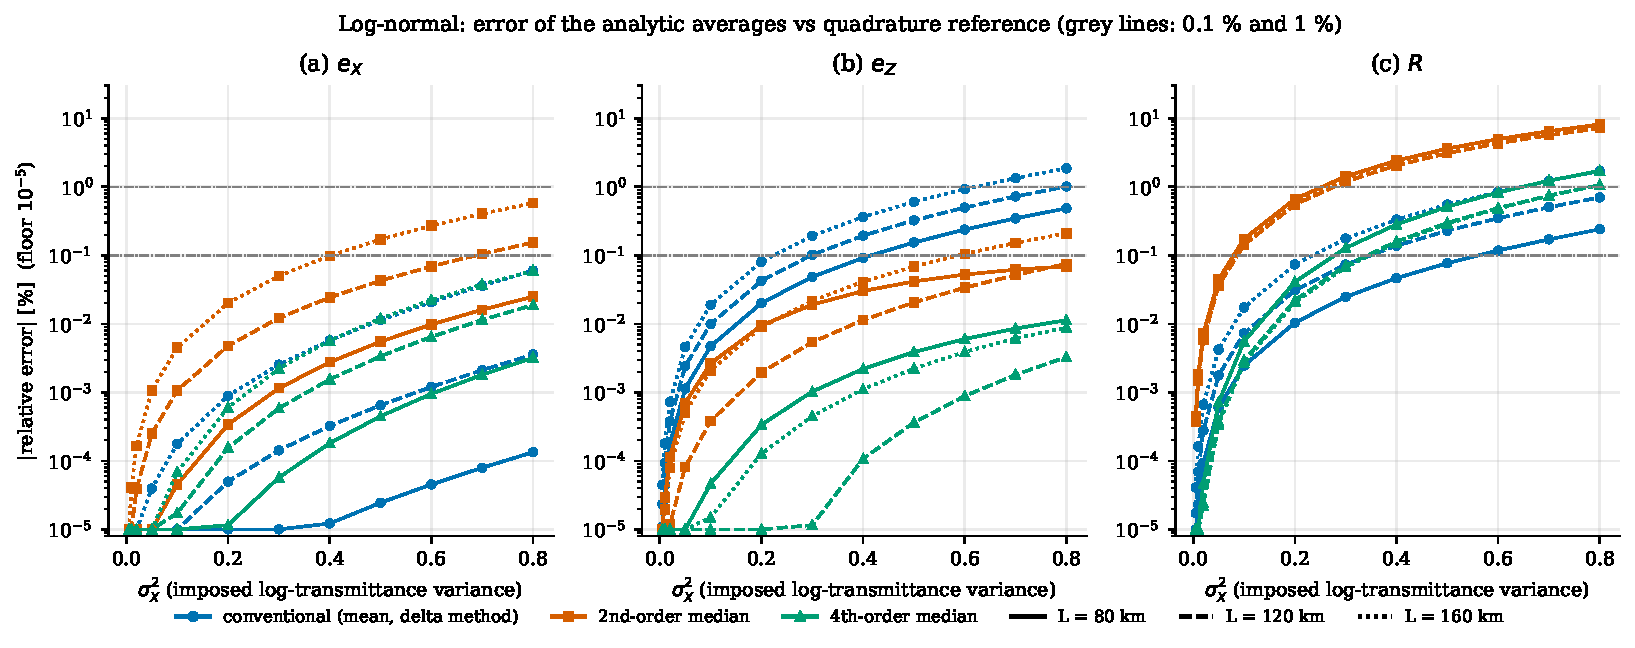
\includegraphics[width=\linewidth]{sens_fig_LN.pdf}\caption{Log-normal channel.}\label{fig:LN}\end{figure}
\begin{figure}[htbp]\centering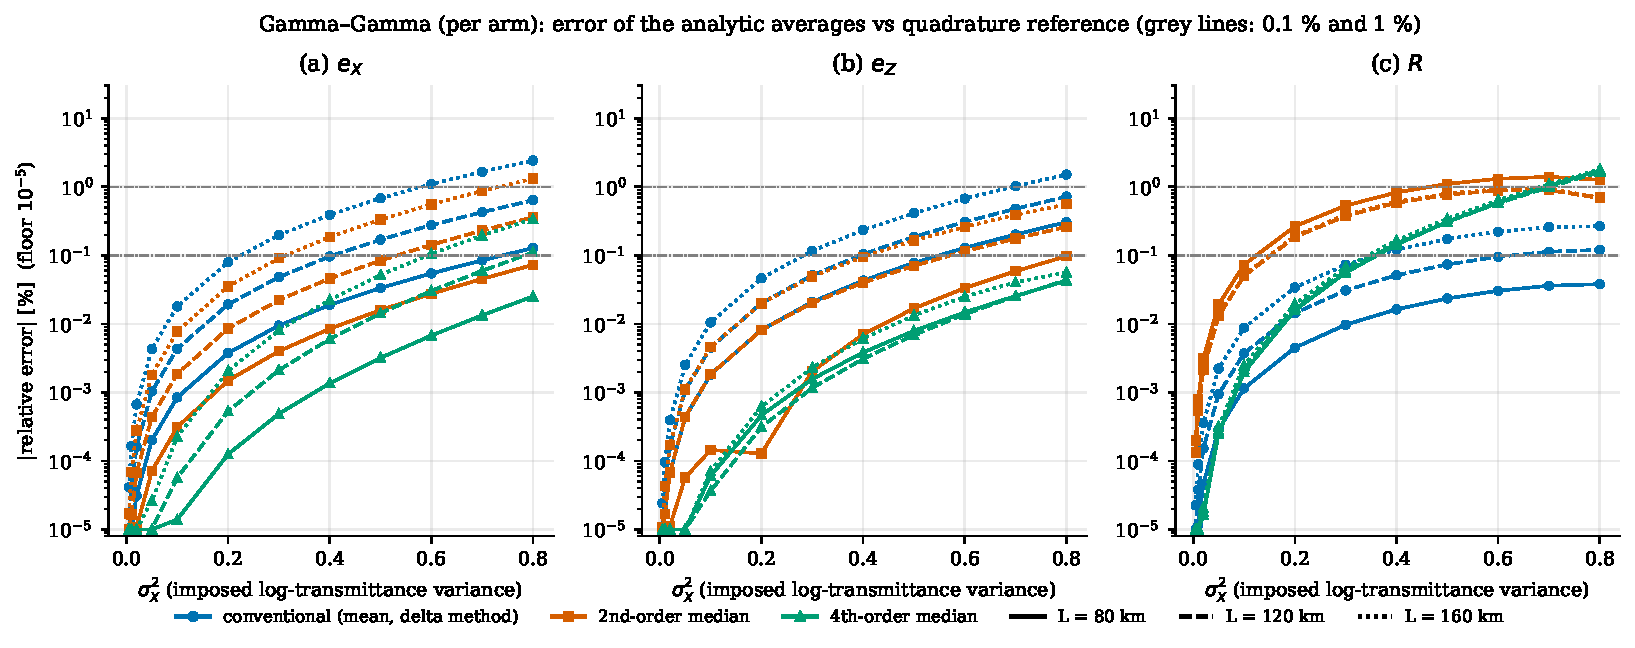
\includegraphics[width=\linewidth]{sens_fig_GG.pdf}\caption{Gamma--Gamma channel (per arm).}\label{fig:GG}\end{figure}
\begin{figure}[htbp]\centering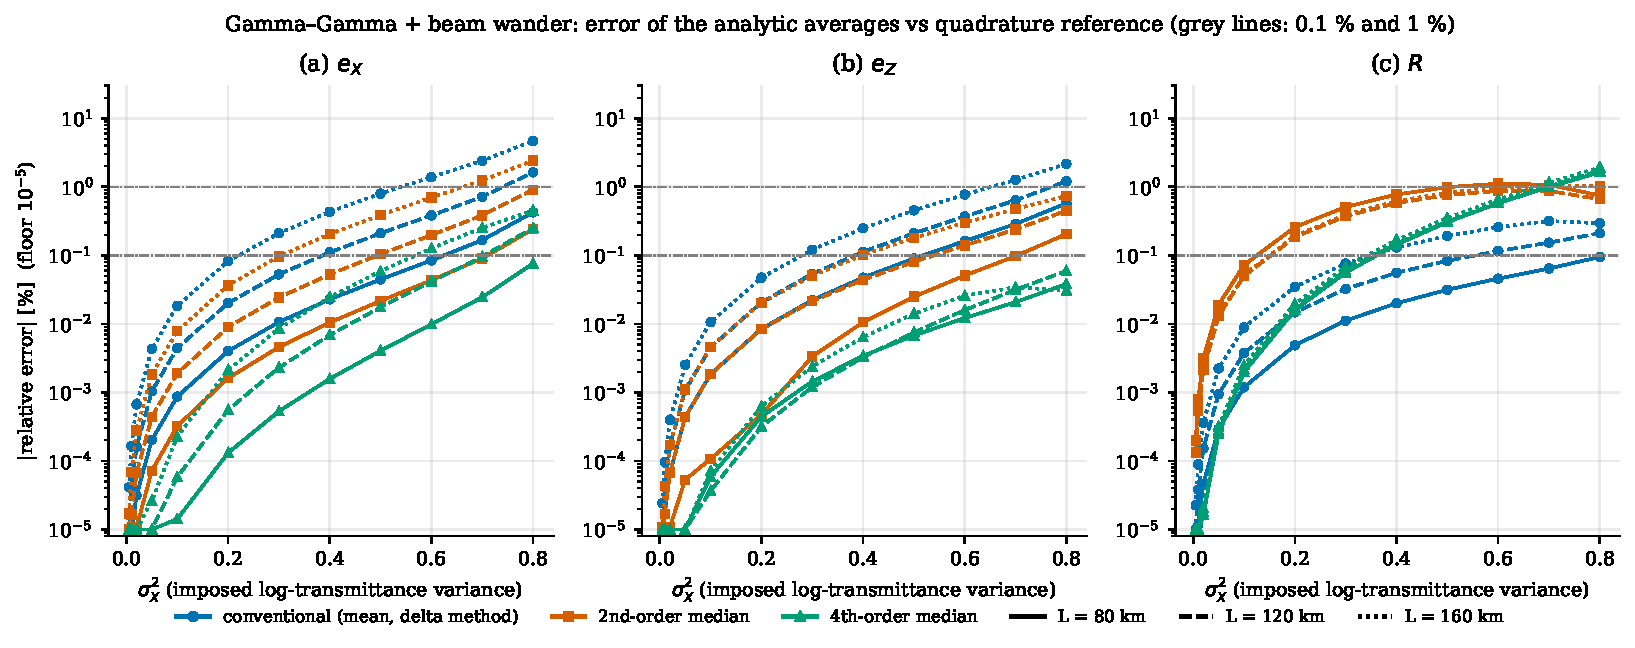
\includegraphics[width=\linewidth]{sens_fig_GGBB.pdf}\caption{Gamma--Gamma channel with beam wander (long-term beam broadening).}\label{fig:GGBB}\end{figure}

\section{Answers established by the data}
\paragraph{1. Does the approximation error increase with turbulence strength?}
Yes, in general. Of the $81$ (model, $L$, quantity, approximation) curves, $72$ increase monotonically in $|{\rm error}|$ over the grid and $9$ do not. The exceptions are the 2nd-order key-rate error of GG and GG+BB at all three distances (six curves; $|{\rm error}|$ peaks at $\sigma_X^2\approx0.6$--$0.7$ and then falls slightly, $1.40\to1.26\%$ at $80$~km for GG), the 2nd-order $e_Z$ of GG at $80$~km, and two small non-monotonicities at GG+BB, $160$~km (mean-approximation $R$, 4th-order $e_Z$). The size and the ranking of the errors depend on the quantity and on the distance (Table~\ref{tab:thr}, \ref{tab:thr2}): errors grow with distance at fixed $\sigma_X^2$ for $e_X$ and $e_Z$ in the GG models (e.g.\ mean-approximation $e_X$ error at $\sigma_X^2=0.8$: $0.13\%$, $0.64\%$, $2.4\%$ at $80,120,160$~km), because the operating point moves to a smaller $\eta_0$ where the error rates vary faster in $\ln\eta$. For $R$ the 4th-order error at $\sigma_X^2=0.8$ is nearly distance independent ($1.6$--$1.9\%$ in GG, $1.1$--$1.7\%$ in LN).

\paragraph{2. When does the 2nd-order approximation become insufficient for the key rate?}
Taking $0.1\%$ as the threshold for a ``precise'' value and $1\%$ for a ``usable'' one: the 2nd-order key-rate error exceeds $0.1\%$ at $\sigma_X^2\approx0.08$--$0.09$ for the log-normal channel and at $0.125$--$0.153$ for Gamma--Gamma, with or without beam wander; it exceeds $1\%$ at $\sigma_X^2\approx0.25$--$0.28$ (LN, all distances) and $0.47$ ($80$~km, GG), $0.51$ (GG+BB, $80$~km), and $0.65$ (GG+BB, $160$~km); for GG at $120$ and $160$~km and GG+BB at $120$~km it stays below $1\%$ up to $0.8$ (maxima $0.89$, $0.93$, $0.87\%$). The log-normal 2nd-order error reaches $7$--$8\%$ at $\sigma_X^2=0.8$. Conclusion: for the key rate the 2nd-order formula stops being accurate (to $0.1\%$) at $\sigma_X^2\approx0.1$, and (to $1\%$) at $\approx0.25$ in log-normal and around $0.5$ or not within the grid in Gamma--Gamma. At the realistic weak-class points ($\sigma_X^2=0.086$--$0.307$ LN, $c_2=0.084$--$0.258$ GG) the 2nd-order key-rate error, interpolated on the grid, is about $0.06$, $0.14$, $0.3\%$ (GG, $80,120,160$~km) and $0.13$, $0.5$, $1.3\%$ (LN).

\paragraph{3. Does the 4th-order approximation stay accurate over the tested range?}
It depends on the quantity.
\begin{itemize}
\item \emph{$e_X$ and $e_Z$:} yes. The 4th-order error stays below $0.46\%$ everywhere and below $0.1\%$ for all LN cases and for GG at $80$~km; its maximum is $0.45\%$ ($e_X$, GG+BB, $160$~km) and $0.06\%$ for $e_Z$. At $\sigma_X^2=0.8$ it is the best of the three approximations for $e_Z$ in every case and for $e_X$ in all GG and GG+BB cases and in LN at $160$~km (in LN at $80$ and $120$~km the mean approximation is marginally better for $e_X$, $\le0.004\%$).
\item \emph{$R$:} the error is bounded ($\le1.9\%$ for $\sigma_X^2\le0.8$) but it is \emph{not} uniformly small. It exceeds $0.1\%$ at $\sigma_X^2\approx0.28$--$0.36$ (LN $0.28$--$0.35$, GG and GG+BB $0.34$--$0.36$) and $1\%$ at $\approx0.65$--$0.78$ (LN $0.65$ at $80$~km and $0.78$ at $120$ and $160$~km; GG and GG+BB $0.68$--$0.70$). In Gamma--Gamma the 4th-order error \emph{overtakes} the 2nd-order one at $\sigma_X^2\approx0.7$ ($L=120,160$~km) and $0.8$ ($80$~km, GG and GG+BB): adding the $\Theta^3,\Theta^4$ terms no longer improves the result, i.e.\ the cumulant series is asymptotic and the third and fourth cumulants are no longer small corrections there. In the log-normal channel the 4th order is better than the 2nd throughout ($1.1$--$1.7\%$ against $7$--$8\%$ at $0.8$).
\item \emph{Surprise in the data:} the conventional mean-transmittance approximation is the \emph{most} accurate for $R$ at $\sigma_X^2=0.8$ in all GG and GG+BB cases ($\le0.30\%$) and in LN at $80$--$120$~km, although it is the worst for $e_X$ and $e_Z$. This is not evidence of a controlled expansion: at these operating points $R(\eta)$ is locally close to a power law ($d\ln R/d\ln\eta=1.05$--$1.13$ at $80$--$160$~km in the repository), for which the curvature correction in $\eta$ is small, and the delta-method error at $160$~km in the log-normal model already grows to $1.7\%$ at $\sigma_X^2=0.8$.
\end{itemize}

\paragraph{Beam wander.} In this controlled setting beam wander only shifts $\eta_0$ by $f_{\rm bb}$ (from $0.999$ to $0.09$--$0.18$ at $\sigma_X^2=0.8$); the key rate itself drops by up to a factor $3.6$ ($2.8$--$3.6$ at $\sigma_X^2=0.8$). The relative errors of $R$ differ from the plain GG case by at most $0.13$ percentage points. The errors of $e_X$ and $e_Z$ grow with the shift towards smaller $\eta_0$, mostly at $160$~km (mean approximation $e_X$ at $\sigma_X^2=0.8$: $2.4\to4.7\%$; 4th order: $0.34\to0.45\%$). The analytic formulas therefore keep their accuracy for the key rate with the beam-wander loss, and lose some for $e_X$ with the conventional approximation, \emph{provided} the shifted operating point stays on the smooth branch of the key-rate curve (all $\eta_m$ here do; $R(\eta_m)\ge6\times10^{-6}$).

\section{Limits}
Only $\sigma_X^2\le0.8$ was tested (the Gamma--Gamma maximum is $0.858$); log-normal behaviour above that, where the repository's validity limit $\sigma_R^2=1$ ($\sigma_X^2=0.5$) is already exceeded for $\sigma_X^2>0.5$, is not covered. The imposed values at fixed distance are a sensitivity device. Error values below $10^{-5}\%$ are plotted at a floor. Reproduction: \texttt{paper\_analysis/scripts/sensitivity\_study.py}, \texttt{sensitivity\_thresholds.py}, \texttt{sensitivity\_figures.py}, \texttt{sensitivity\_make\_tex.py} (they import the repository unchanged).
\end{document}
